\documentclass[10pt,twocolumn,letterpaper]{article}

\usepackage{cvpr}
\usepackage{xfrac}
\usepackage{times}
\usepackage{epsfig}
\usepackage{graphicx}
\usepackage{listings}
\usepackage{amsmath}
\usepackage{amssymb}
\usepackage{color, soul}
\usepackage{float}
\usepackage[super]{nth}
\setlength{\intextsep}{5pt}
\usepackage[nodisplayskipstretch]{setspace}
\setstretch{1}
\usepackage{algorithm}
\usepackage{algorithmic}
\usepackage[utf8]{inputenc}

% Include other packages here, before hyperref.

% If you comment hyperref and then uncomment it, you should delete
% egpaper.aux before re-running latex.  (Or just hit 'q' on the first latex
% run, let it finish, and you should be clear).
\usepackage[breaklinks=true,bookmarks=false]{hyperref}

\cvprfinalcopy % *** Uncomment this line for the final submission

\def\cvprPaperID{****} % *** Enter the CVPR Paper ID here
\def\httilde{\mbox{\tt\raisebox{-.5ex}{\symbol{126}}}}

% Pages are numbered in submission mode, and unnumbered in camera-ready
%\ifcvprfinal\pagestyle{empty}\fi
\setcounter{page}{1}
\begin{document}

%%%%%%%%% TITLE
\title{Pattern Recognition Coursework 2}

\author{Jakub Mateusz Szypicyn\\
CID: 00846006\\
EEE4\\
{\tt\small jms13@ic.ac.uk}
% For a paper whose authors are all at the same institution,
% omit the following lines up until the closing ``}''.
% Additional authors and addresses can be added with ``\and'',
% just like the second author.
% To save space, use either the email address or home page, not both
\and
Jacobus Jukka Hertzog\\
CID: 00828711\\
EEE4\\
{\tt\small jjh13@ic.ac.uk}
}

\maketitle
%\thispagestyle{empty}

%%%%%%%%% ABSTRACT
\begin{abstract}
Line 1\\

Line 2\\

Line 3\\
\end{abstract}

\section{Introduction}
\section{Distance Metrics}
\subsection{Distribution of Wine Data}

The wine data ({\tt\small wine.csv}) provided consisted of three classes. It cis made up of 13 features representing chemical and optical information. The data can be analysed \textit{talis qualis}, however a more elaborate method is to investigate the covariance matrices. The raw data can supply us with information such as feature distribution (mean or spread), whereas covariance matrices will provide the dependency between features. This can be performed for all data altogether or for each class individually. Both methods will result in meaningful information as described in sections \ref{sec:CovAll} and \ref{sec:CovCla}. Furthermore the data was then normalised and the above was repeated.\footnote{Note that data was first separated as per instruction. Only training data is now being considered.} 
\subsubsection{All Classes} \label{sec:CovAll}
By investigating the data from all classes we will see that data varies altogether. We can investigate each feature and see what part of space it occupies. We can also determine how strongly all features are related to one another for all classes. Let us begin by examining the distributions of the raw data. The means of the feature distributions vary from around 0.36 for nonflavanoid phenols, through values of 1 to 3 and 10 to 100 to a single extreme at 737.1 for proline. The corresponding deviations are also quite spread out. The general trend is that the larger the mean the larger the standard deviation of the distribution. For example proline distribution has a standard deviation of 287 over 118 samples. The distributions of the features don't always seem to follow bell-shaped Gaussian distribution. However it should be noted that each distribution is in fact a sum of three independent distributions. Distribution of proline in Figure \ref{fig:DistProline} resembles a gamma distribution.

\begin{figure}[H]
\centering
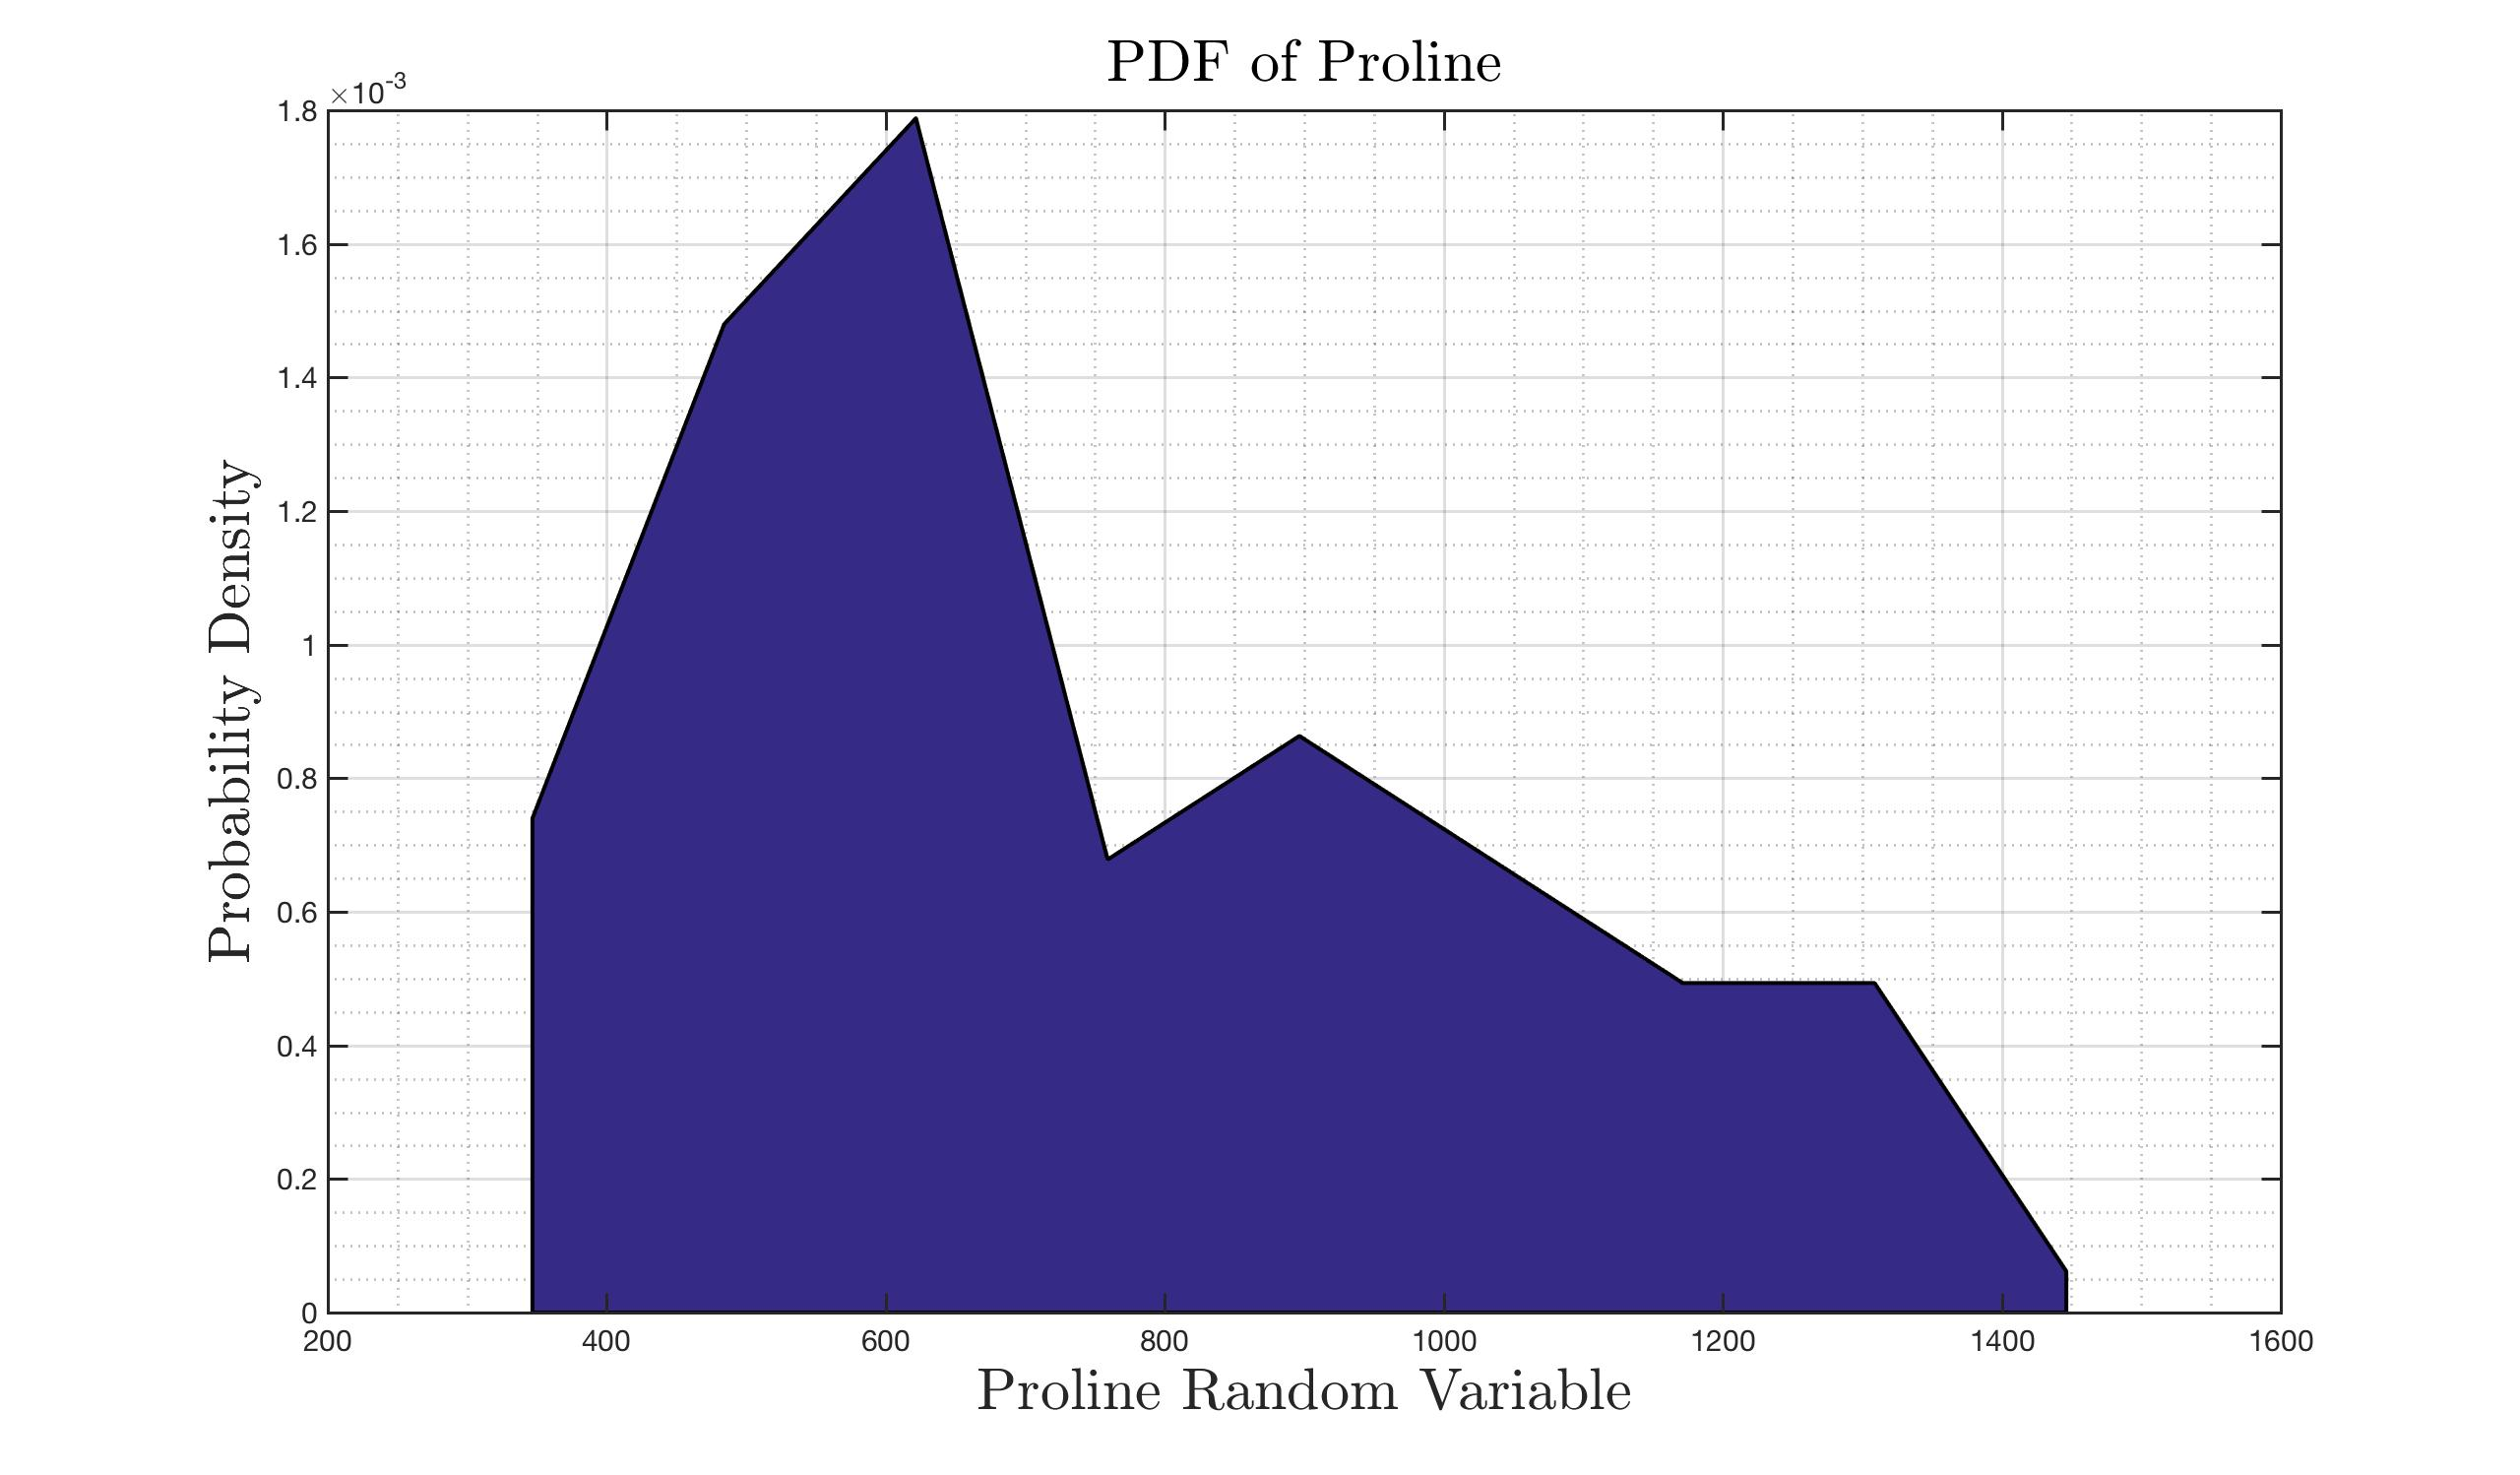
\includegraphics[width=0.4\textwidth]{../results/Q1_ProlineDist}
\caption{Distribution of Proline from all Classes \label{fig:DistProline}}
\end{figure}

\begin{table}[H]
\caption{Sample Means and Standard Dev. for all Training Data}
\begin{center}
\begin{tabular}{|c c c c c|}
\hline
\bf RV & Alcohol & Ash & Hue & Proline \\ [0.5ex]
\hline
\bf Mean & 12.7 & 2.38 & 0.95 & 737 \\ [0.5ex]
\hline
\bf Std. & 0.72 & 0.29 & 0.24 & 287 \\ [0.5ex]
\hline
\end{tabular}
\end{center}
\end{table}

Looking at the covariance matrix of the raw training data we can see that proline covary with all other features quite strongly. This is however due to the fact that proline's distribution has a naturally high variance, thus corrupting the readings. The highest covariance for two different features excluding proline is that of magnesium (feature 5) and colour intensity (feature 10). However, these two features have second and third highest variance distributions. We have to therefore look at the covariance matrix of the normalised feature vectors.

Highest positive covariance is observed for features 6 and 7 (total phenols and flavanoids), whereas the most negative covariance is found for features 2 and 7 (malic acid and flavanoids). The plot of the above cases is shown in Figure \ref{fig:covAll}.

\begin{figure}[H]
\centering
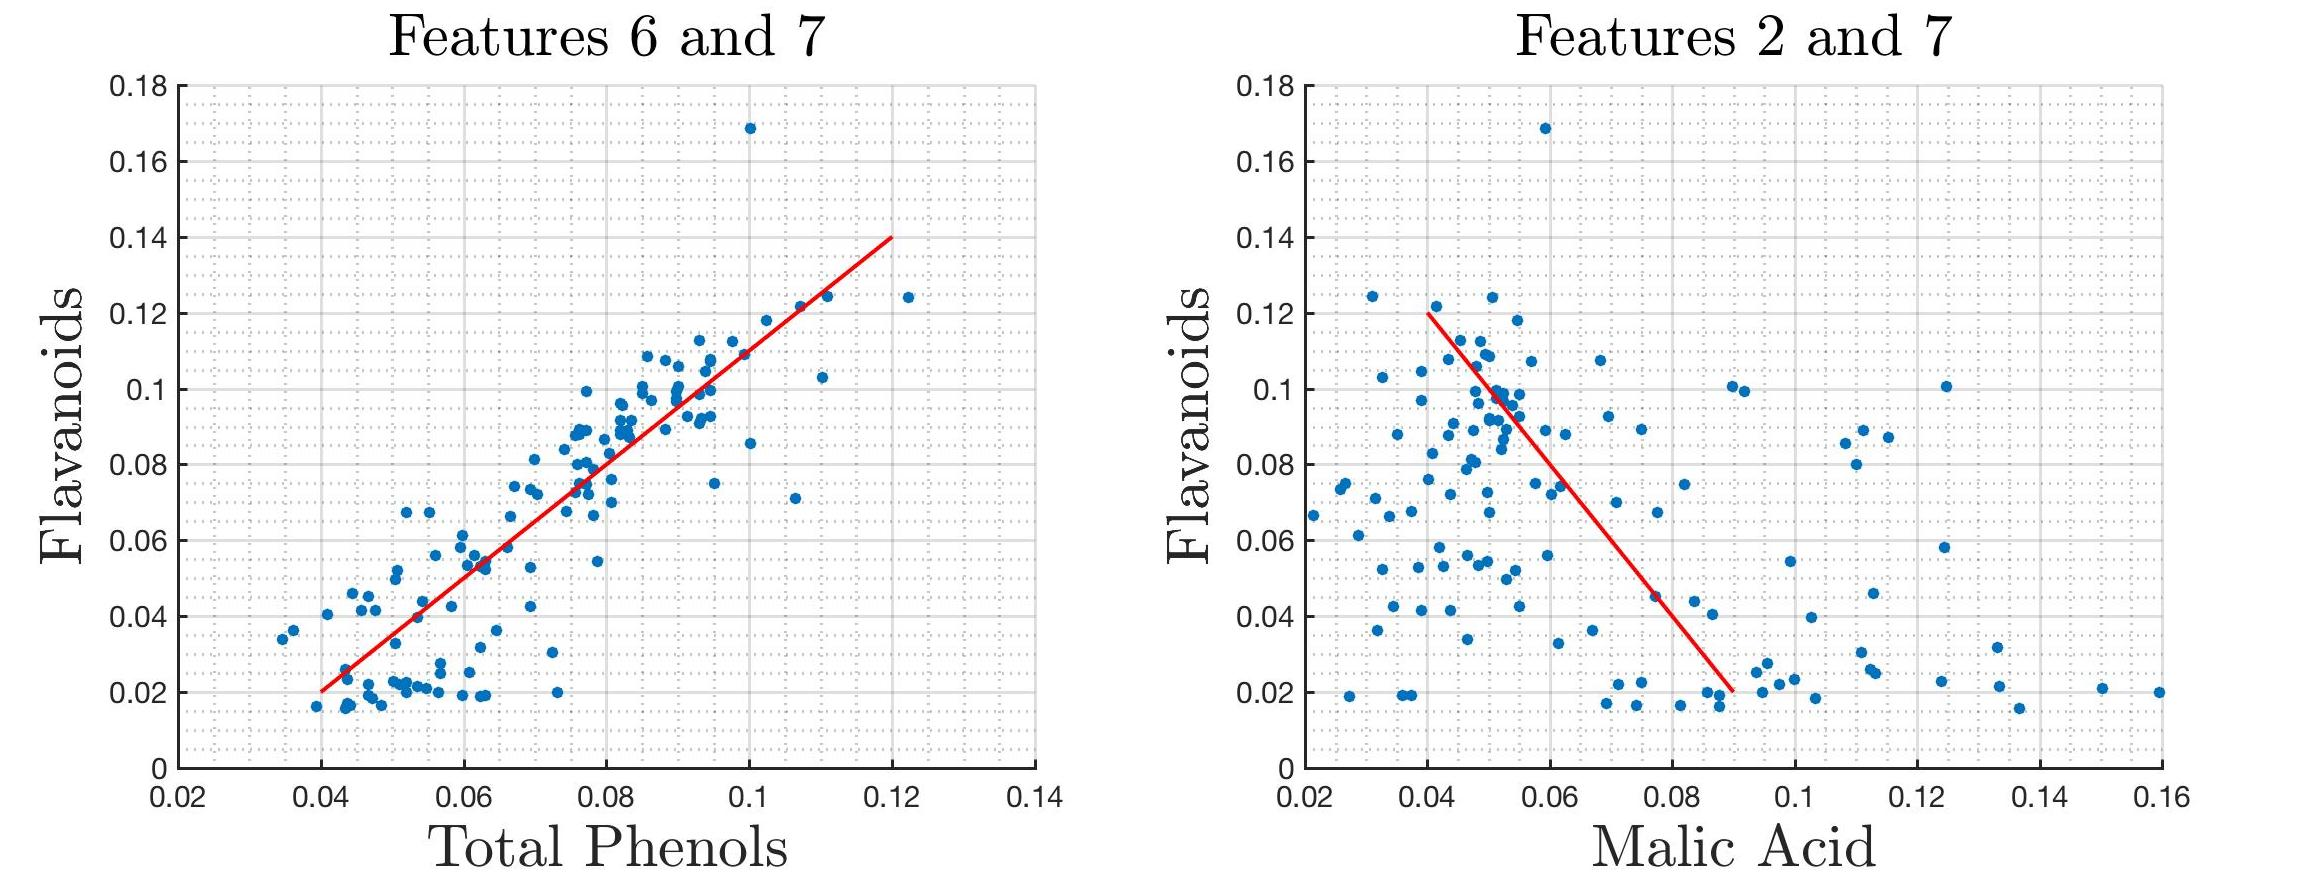
\includegraphics[width=0.5\textwidth]{../results/Q1_covAll}
\caption{Covariance of Features 6 \& 7 and 2 \& 7 Visualised \label{fig:covAll}}
\end{figure}

\subsubsection{Individual Classes} \label{sec:CovCla}

\subsection{L1 and L2 Metrics}

\subsection{Chi-Squared and Correlation Metrics}

\subsection{Histogram Intersection Metric}

\subsection{Mahalanobis Distance Metric}

\section{K-means Clustering}

\section{Neural Network}

\section{Conclusion}
\end{document}
